\chapter{Arhitektura i dizajn sustava}

	Aplikacija se sastoji od tri podsustava:
	
		\begin{itemize}
			\item Preglednik
			\item Poslužitelj
			\item Baza podataka
		\end{itemize}
	
	Putem preglednika korisnici pristupaju aplikaciji te šalju ili primaju podatke od poslužitelja. Odabrani protokol za komunikaciju između korisnika i aplikacije je HTTP protokol. Za rad na pregledniku odabrana je tehnologija React.
	
	Poslužitelj prihvaća zahtjeve korisnika te šalje informacije nazad na preglednik koji se prikazuju korisniku. Poslužitelj također pristupa bazi podataka te obrađuje podatke koji se nalaze u bazi. Poslužitelj se radi u Java Spring frameworku.
	
	Arhitektura sustava je zasnovana na modelu Model View Component.
	
	
	
	
	
	
	\section{Baza podataka}
		
		
	Odabrana je relacijska baza podataka implementirana pomoću PostgreSQL. Baza podataka je normalizirana te je u trećoj normalnoj formi. Sastavljena je od entiteta
			\begin{itemize}
				\item korisnik
				\item spasilac
				\item dispečer
				\item akcija
				\item stanica
				\item način spašavanja
				\item zadatak
			\end{itemize}
		
			\subsection{Opis tablica}
			
				\begin{longtabu} to \textwidth {|X[7, l]|X[7, l]|X[20, l]|}
					
					\hline \multicolumn{3}{|c|}{\textbf{KORISNIK}}	 \\[3pt] \hline
					\endfirsthead
					
					\hline \multicolumn{3}{|c|}{\textbf{KORISNIK}}	 \\[3pt] \hline
					\endhead
					
					\hline 
					\endlastfoot
					
					\textbf{korisnickoIme} & VARCHAR	&  	Jedinstveno korisničko ime svakog korisnika 	\\ \hline
					lozinka	& VARCHAR & lozinka korisnika	\\ \hline 
					ime & VARCHAR	&  		\\ \hline 
					prezime & VARCHAR & \\ \hline
					brojMob & VARCHAR & broj mobitela korisnika \\ \hline
					email & VARCHAR & email korisnika \\ \hline
					uloga & VARCHAR & varijabla koja služi u backend dijelu za dodjeljivanje u određenu tablicu(spasilac/dispečer) \\ \hline
					status & VARCHAR & status je li korisnik registriran ili nije \\ \hline
					
					
				\end{longtabu}
				
				\begin{longtabu} to \textwidth {|X[7, l]|X[7, l]|X[20, l]|}
					
					\hline \multicolumn{3}{|c|}{\textbf{DISPEČER}}	 \\[3pt] \hline
					\endfirsthead
					
					\hline \multicolumn{3}{|c|}{\textbf{DISPEČER}}	 \\[3pt] \hline
					\endhead
					
					\hline 
					\endlastfoot
					
					\textbf{korisnickoIme} & VARCHAR	&  	Ujedno i strani ključ na tablicu korisnik, u tablici se spremaju svi korisnici koji su dispečeri 	\\ \hline
					
					
				\end{longtabu}
				
				\begin{longtabu} to \textwidth {|X[7, l]|X[7, l]|X[20, l]|}
					
					\hline \multicolumn{3}{|c|}{\textbf{SPASILAC}}	 \\[3pt] \hline
					\endfirsthead
					
					\hline \multicolumn{3}{|c|}{\textbf{SPASILAC}}	 \\[3pt] \hline
					\endhead
					
					\hline 
					\endlastfoot
					
					\textbf{korisnickoIme} & VARCHAR	&  	Ujedno i strani ključ na tablicu korisnik, u tablici se spremaju svi korisnici koji su spasioci 	\\ \hline
					\textit{sifStanica} & VARCHAR & Šifra stanice kojoj pripada spasilac \\ \hline
					dostupan & BOOLEAN & Je li spasilac dostupan za odazivanje na akciju \\ \hline
					
				\end{longtabu}
				
				\begin{longtabu} to \textwidth {|X[7, l]|X[7, l]|X[20, l]|}
					
					\hline \multicolumn{3}{|c|}{\textbf{STANICA}}	 \\[3pt] \hline
					\endfirsthead
					
					\hline \multicolumn{3}{|c|}{\textbf{STANICA}}	 \\[3pt] \hline
					\endhead
					
					\hline 
					\endlastfoot
					
					\textbf{sifStanica} & VARCHAR	&  	Jedinstvena šifra stanice 	\\ \hline
					nazivStanica & VARCHAR & Ime stanice \\ \hline
					\textit{korImeVoditelj} & VARCHAR & Korisničko ime spasioca koji je voditelj stanice \\ \hline
					
				\end{longtabu}
				
				\begin{longtabu} to \textwidth {|X[7, l]|X[7, l]|X[20, l]|}
					
					\hline \multicolumn{3}{|c|}{\textbf{AKCIJA}}	 \\[3pt] \hline
					\endfirsthead
					
					\hline \multicolumn{3}{|c|}{\textbf{AKCIJA}}	 \\[3pt] \hline
					\endhead
					
					\hline 
					\endlastfoot
					
					\textbf{sifAkcija} & VARCHAR	&  	Jedinstvena šifra akcije 	\\ \hline
					nazivAkcija & VARCHAR & Ime akcije \\ \hline
					infNestalaOsoba & VARCHAR & Kratki opis i informacije o nestaloj osobi \\ \hline
					lokacija & VARCHAR & Lokacija potrage \\ \hline
					\textit{korImeDispečer} & VARCHAR & Dispečer koji koordinira akciju \\ \hline
					status & VARCHAR & Status akcije (u tijeku/završena) \\ \hline
					
				\end{longtabu}
				
				\begin{longtabu} to \textwidth {|X[7, l]|X[7, l]|X[20, l]|}
					
					\hline \multicolumn{3}{|c|}{\textbf{ZADATAK}}	 \\[3pt] \hline
					\endfirsthead
					
					\hline \multicolumn{3}{|c|}{\textbf{ZADATAK}}	 \\[3pt] \hline
					\endhead
					
					\hline 
					\endlastfoot
					
					\textbf{sifZadatak} & VARCHAR & Jedinstvena šifra zadatka \\ \hline
					nazivZadatak & VARCHAR & Naziv zadatka \\ \hline
					\textit{korImeDispecer} & VARCHAR & Dispečer koji je spasiocu zadao zadatak \\ \hline
					\textit{korImeSpasilac} & VARCHAR & Spasilac kojem je zadan zadatak \\ \hline
					komentar & VARCHAR & Komentar za određeni zadatak \\ \hline
					
					
				\end{longtabu}
				
				\begin{longtabu} to \textwidth {|X[7, l]|X[7, l]|X[20, l]|}
					
					\hline \multicolumn{3}{|c|}{\textbf{SPASILACAKCIJA}}	 \\[3pt] \hline
					\endfirsthead
					
					\hline \multicolumn{3}{|c|}{\textbf{SPASILACAKCIJA}}	 \\[3pt] \hline
					\endhead
					
					\hline 
					\endlastfoot
					
					\textbf{korImeSpasilac} & VARCHAR & Korisničko ime spasioca na određenoj akciji \\ \hline
					\textit{sifAkcija} & VARCHAR & Šifra akcije na kojoj sudjeluje određeni spasilac
					
					
				\end{longtabu}
				
				\begin{longtabu} to \textwidth {|X[7, l]|X[7, l]|X[20, l]|}
					
					\hline \multicolumn{3}{|c|}{\textbf{SPASILACAKCIJA}}	 \\[3pt] \hline
					\endfirsthead
					
					\hline \multicolumn{3}{|c|}{\textbf{SPASILACAKCIJA}}	 \\[3pt] \hline
					\endhead
					
					\hline 
					\endlastfoot
					
					\textbf{korImeSpasilac} & VARCHAR & Korisničko ime spasioca na određenoj akciji \\ \hline
					\textit{sifAkcija} & VARCHAR & Šifra akcije na kojoj sudjeluje određeni spasilac 
					
					
				\end{longtabu}
			
				\begin{longtabu} to \textwidth {|X[7, l]|X[7, l]|X[20, l]|}
					
					\hline \multicolumn{3}{|c|}{\textbf{NACINSPASAVANJA}}	 \\[3pt] \hline
					\endfirsthead
					
					\hline \multicolumn{3}{|c|}{\textbf{NACINSPASAVANJA}}	 \\[3pt] \hline
					\endhead
					
					\hline 
					\endlastfoot
					
					\textbf{sifNacin} & VARCHAR & Šifra načina spašavanja \\ \hline
					imeNacin & VARCHAR & Naziv načina spašavanja \\ \hline
					intenzitet & INT & Kolikim intenzitetom se može tragati s ovakvim načinom \\ \hline
					velicina & INT & Koliko područje se može pretražiti s ovakvim načinom	\\ \hline			 	
					
					
				\end{longtabu}
			
				\begin{longtabu} to \textwidth {|X[7, l]|X[7, l]|X[20, l]|}
					
					\hline \multicolumn{3}{|c|}{\textbf{ZAHTJEV}}	 \\[3pt] \hline
					\endfirsthead
					
					\hline \multicolumn{3}{|c|}{\textbf{ZAHTJEV}}	 \\[3pt] \hline
					\endhead
					
					\hline 
					\endlastfoot
					
					\textbf{sifAkcija} & VARCHAR & Korisničko ime spasioca na određenoj akciji \\ \hline
					\textbf{sifStanica} & VARCHAR & Šifra akcije na kojoj sudjeluje određeni spasilac \\ \hline
					\textit{sifNacin} & VARCHAR & Način spašavanja koji se zahtijeva od određene stanice \\ \hline
					
				\end{longtabu}
			
				\begin{longtabu} to \textwidth {|X[7, l]|X[7, l]|X[20, l]|}
					
					\hline \multicolumn{3}{|c|}{\textbf{SPASILACNACIN}}	 \\[3pt] \hline
					\endfirsthead
					
					\hline \multicolumn{3}{|c|}{\textbf{SPASILAC}}	 \\[3pt] \hline
					\endhead
					
					\hline 
					\endlastfoot
					
					\textbf{korImeSpasilac} & VARCHAR & Korisničko ime spasioca na određenoj akciji \\ \hline
					\textbf{sifNacin} & VARCHAR & Šifra načina na koje sve može određeni spasilac sudjelovati u akciji \\ \hline
					
					
				\end{longtabu}
		
		\subsection{Dijagram baze podataka}
		\begin{figure}[h!]
			\centering
			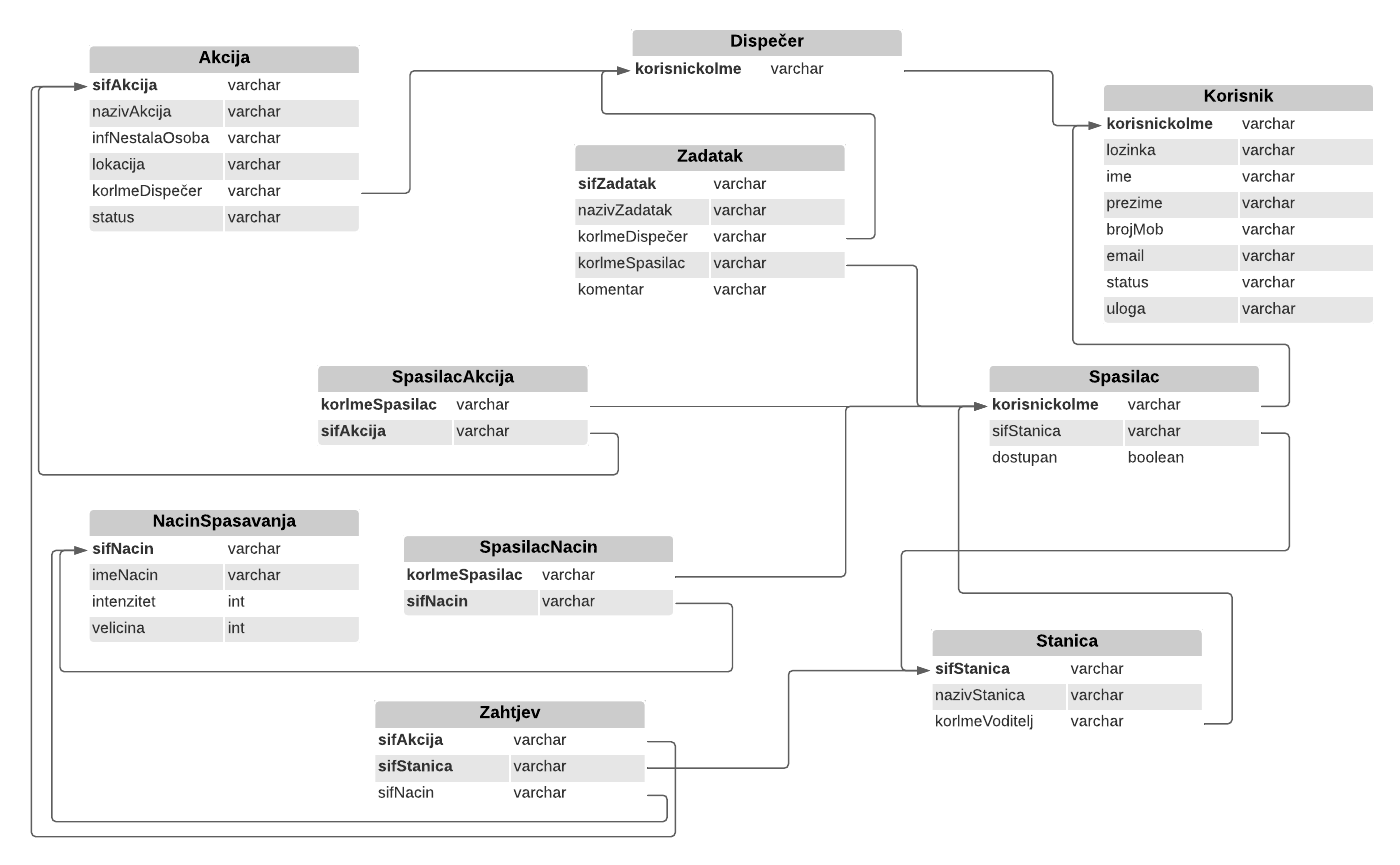
\includegraphics[width=\textwidth]{./slike/dijagrambaze.png}
			\caption{Dijagram baze podataka}
			
		\end{figure}
		
		\eject
	
	
	\section{Dijagram razreda\\}
	
	
	{Na priloženim slikama moguće je vidjeti dijagrame razreda \textit{backend} dijela MVC \\arhitekture.\\}
	
	
	{Na slici 4.2 je prikazana \textbf{Application Controller} klasa  koja se sastoji od metoda koje koriste metode iz \textbf{KorisnikDao}  klase, koja  služi za pristup podataka iz baze sustava.Klasi KorisnikDao controller  pristupa preko funkcija iz \textbf{KorisnikService} klase}\\
	
	\begin{figure}[h!]
		\centering
		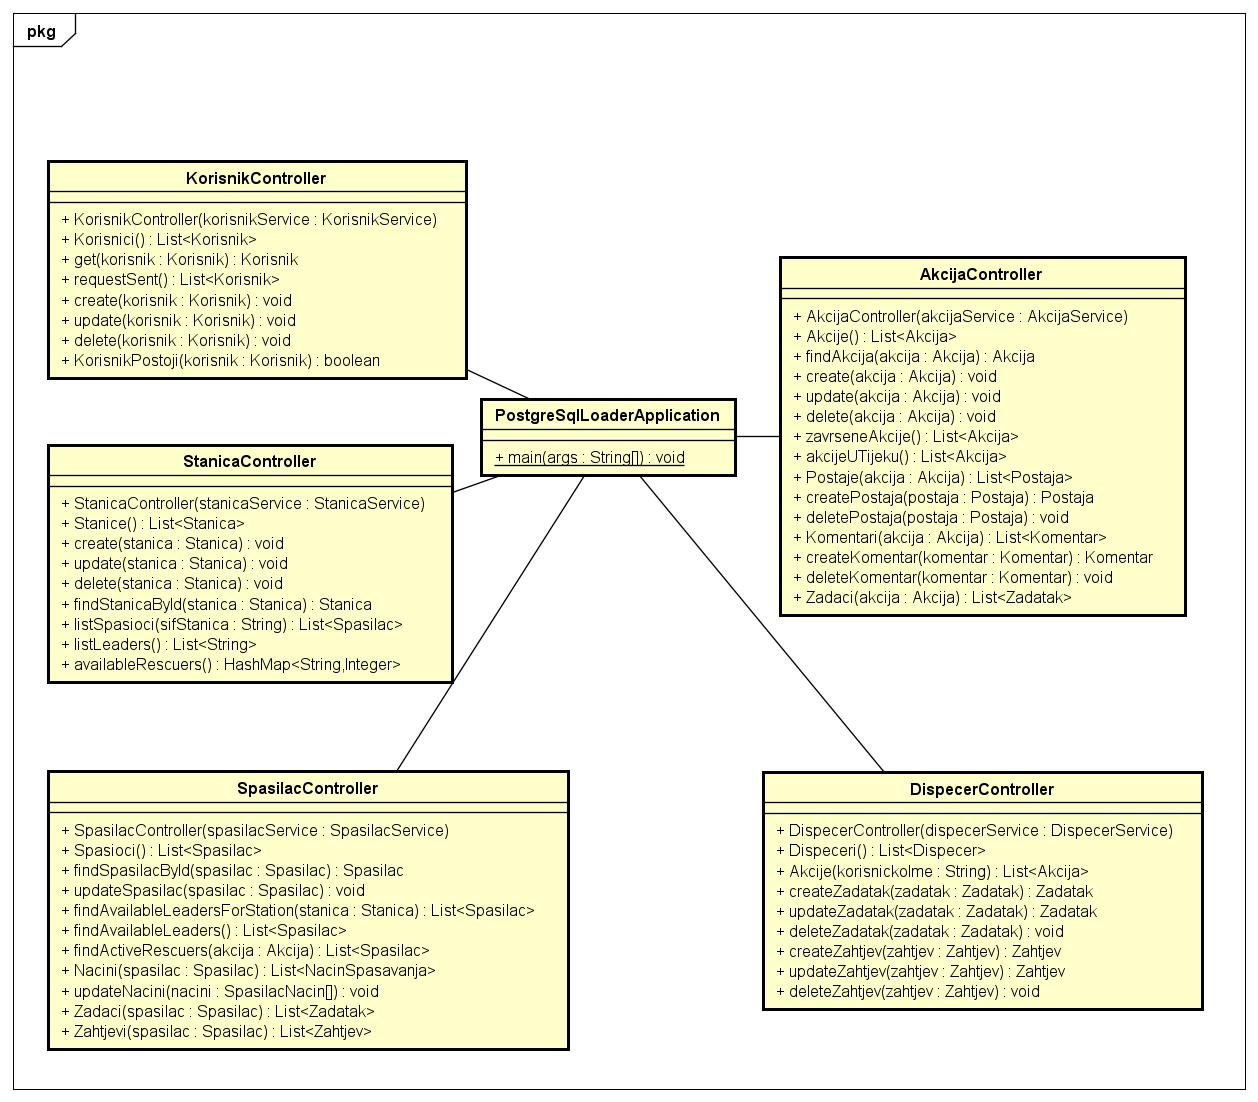
\includegraphics[width = \linewidth]{./slike/Controllers.jpg}
		\caption{Prikaz klase AplicationController}
		
	\end{figure}
	\newpage
	
	{Slika 4.3 prikazuje klase \textbf{Service} te klase \textbf{ServiceImpl} }
	{koje služe za prikaz entiteta kroz bazu za manipuliranje podatcima.\newline Slika također prikazuje ovisnost Sve ove klase se služe klasom entiteta istog imena koja omogućuje prikaz te manipulaciju s podatcima iz baze podataka.\\}\\
	
	\begin{figure}[h!]
		\centering
		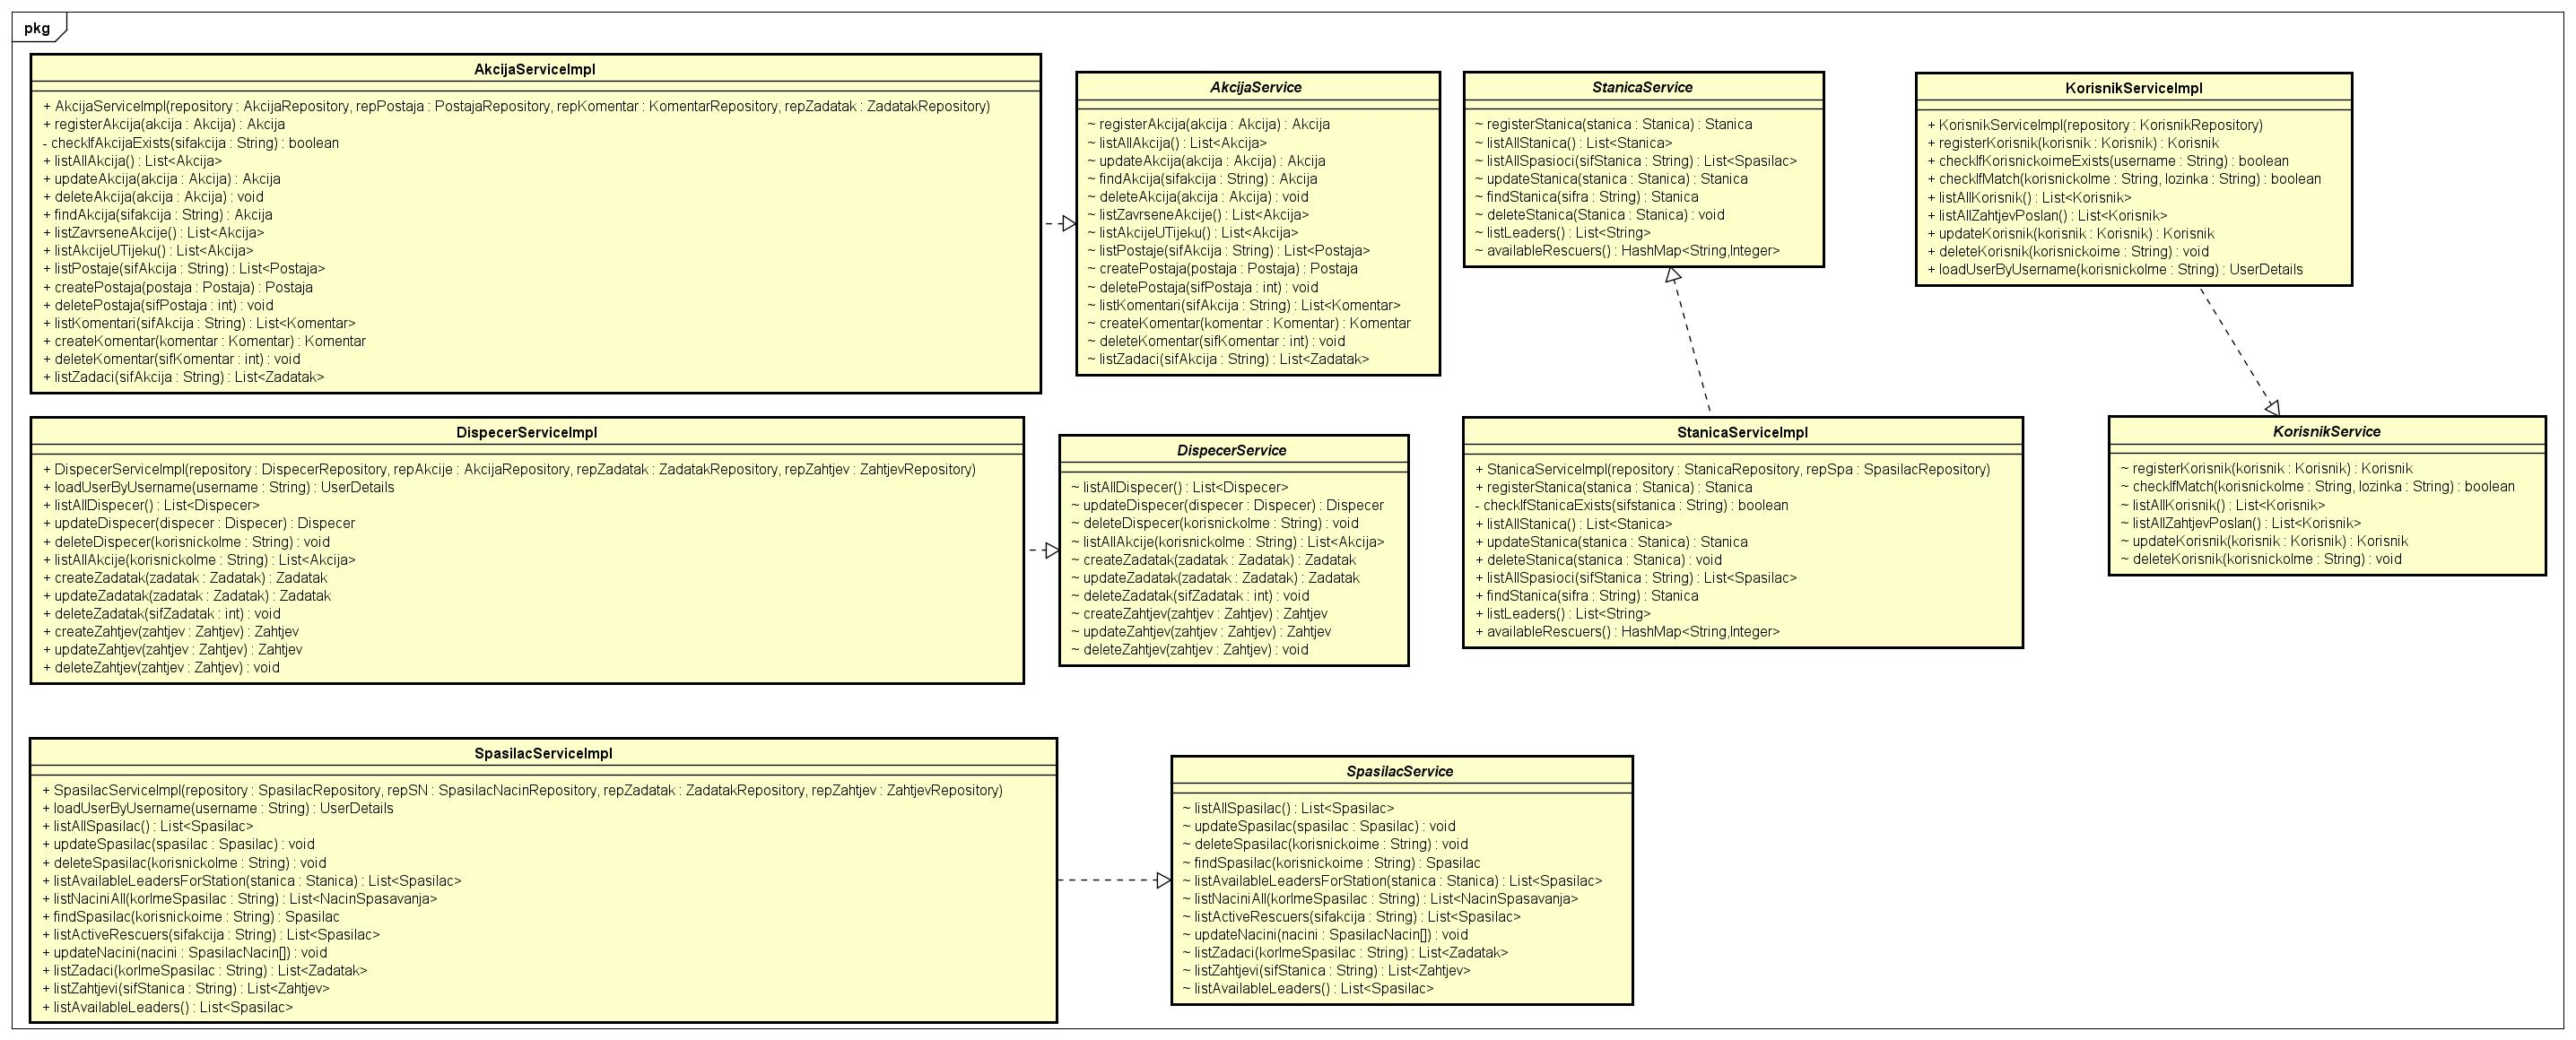
\includegraphics[width=\linewidth]{./slike/ServisImpl.jpg}
		\caption{Prikaz klasa servisa te klasa vezanih uz njihovu implementaciju}
		
	\end{figure}	
	\newpage
	{Za pristup bazi podataka te podatcima u njoj koriste se klase \textbf{Entity} koje koriste \textbf{JPA} funkcije za manipuliranje podataka. Na temelju entitet klasa u kojima podatci moraju biti navedeni istim redoslijedom kao i u bazi podataka funkcije pretražuju podatke.Entiteti aplikacije prikazani su na slici 4.4\\}
	
	\begin{figure}[h!]
		\centering
		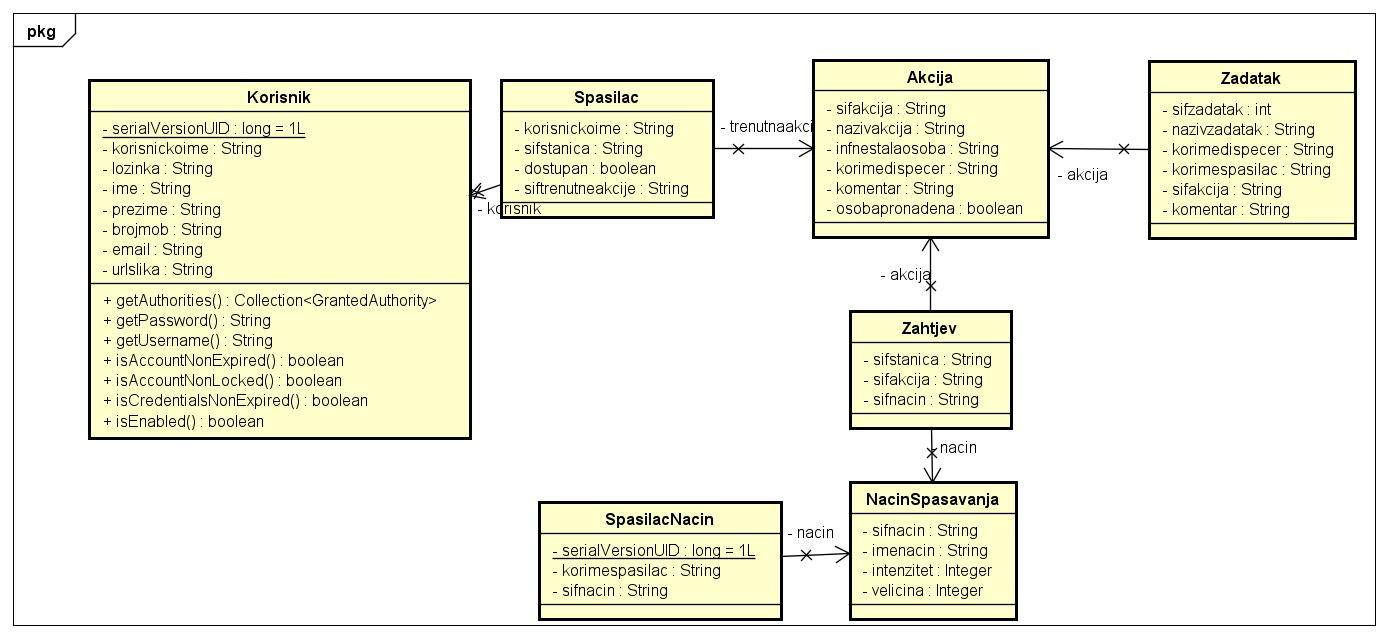
\includegraphics[width=\linewidth]{./slike/Entiteti.jpg}
		\caption{Prikaz klasa Entiteta koji su apstraktni prikazi podataka u bazi podataka}
		
	\end{figure}

	\eject
	
	\newpage
	\section{Dijagram stanja}
	
		{Dijagram stanja prikazuje stanja objekta te prijelaze iz jednog stanja u drugo temeljene na događajima. Na slici 4.5 prikazan je dijagram stanja za spasioca čiji su podatci prethodno potvrđeni od strane admina. Pri prijavi spasiocu se prikazuje početna stranica iz koje može prijeći na neko od drugih stanja(dijelova aplikacije). Za karticu "Trenutna akcija" spasilac može ostaviti komentare na akciju, postaviti privremenu postaju, te javiti dispečeru da je tražena žrtva pronađena. Za karticu "Akcije u tijeku" spasilac može vidjeti koje su trenutačno aktivne akcije na koje se može dobrovoljno prijaviti. Spasilac također ima i mogućnost vidjeti jesu li mu poslani zahtjevi za prijavu na neku od akcija,gumb "Pregled zahtjeva za spasioce",gdje su zahtjevi slani od strane dispečera ili voditelja stanice spasioca. Klikom na "Profil" spasilac ima mogućnost mijenjanja vlastitih osobnih podataka, brisanja svojega računa ako nema potrebu ili ne želi koristiti aplikaciju u budućnosti te javljanja svojeg trenutnog stanja (dostupnost za akcije).}
	
		\begin{figure}[h!]
			\centering
			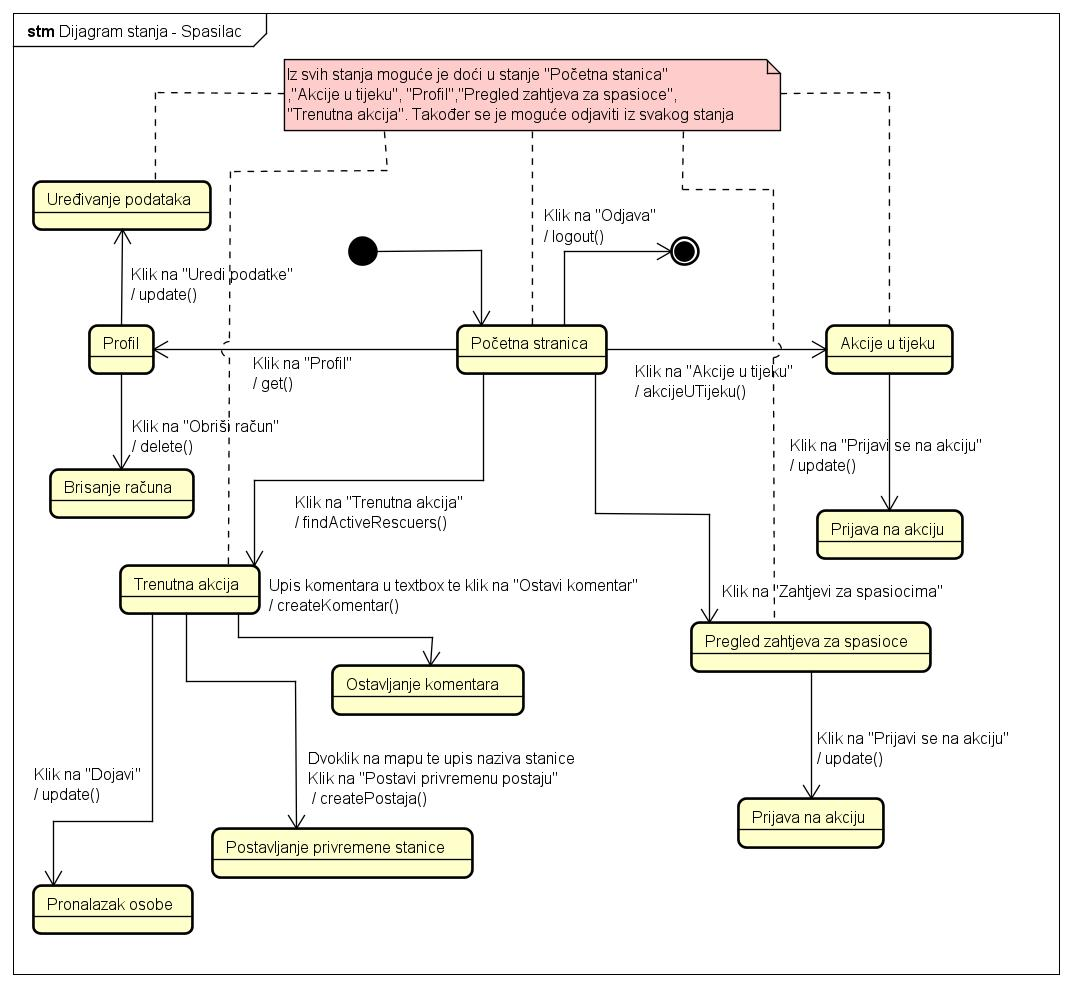
\includegraphics[width=\linewidth]{./slike/Dijagram stanja - Spasilac.jpg}
			\caption{Prikaz dijagrama stanja}
		
		\end{figure}
	
	
	\eject 
	
	\section{Dijagram aktivnosti}
	
 	\begin{packed_item}
		\item	{Dijagram aktivnosti primjenjuje se za opis modela toka upravljanja ili toka podataka za pregled na aplikaciji. U modeliranju toka upravljanja svaki korak obavlja se nakon završetka koraka koji mu prethodi s naglaskom na jednostavnost. Na dolje prikazanim dijagramima (slike 4.6 i 4.7) prikazani su razni procesi koje aplikacija izvodi ovisno o traženim upitima korisnika.\\
			Slika 4.6 prikazuje proces javljanja spasioca na akciju. Korisnik se prijavi u sustav, potom izabire jednu od trenutno aktivnih akcija spašavanja te klikom na gumb se prijavljuje u istu}
		
		\begin{figure}[h!]
			\centering
			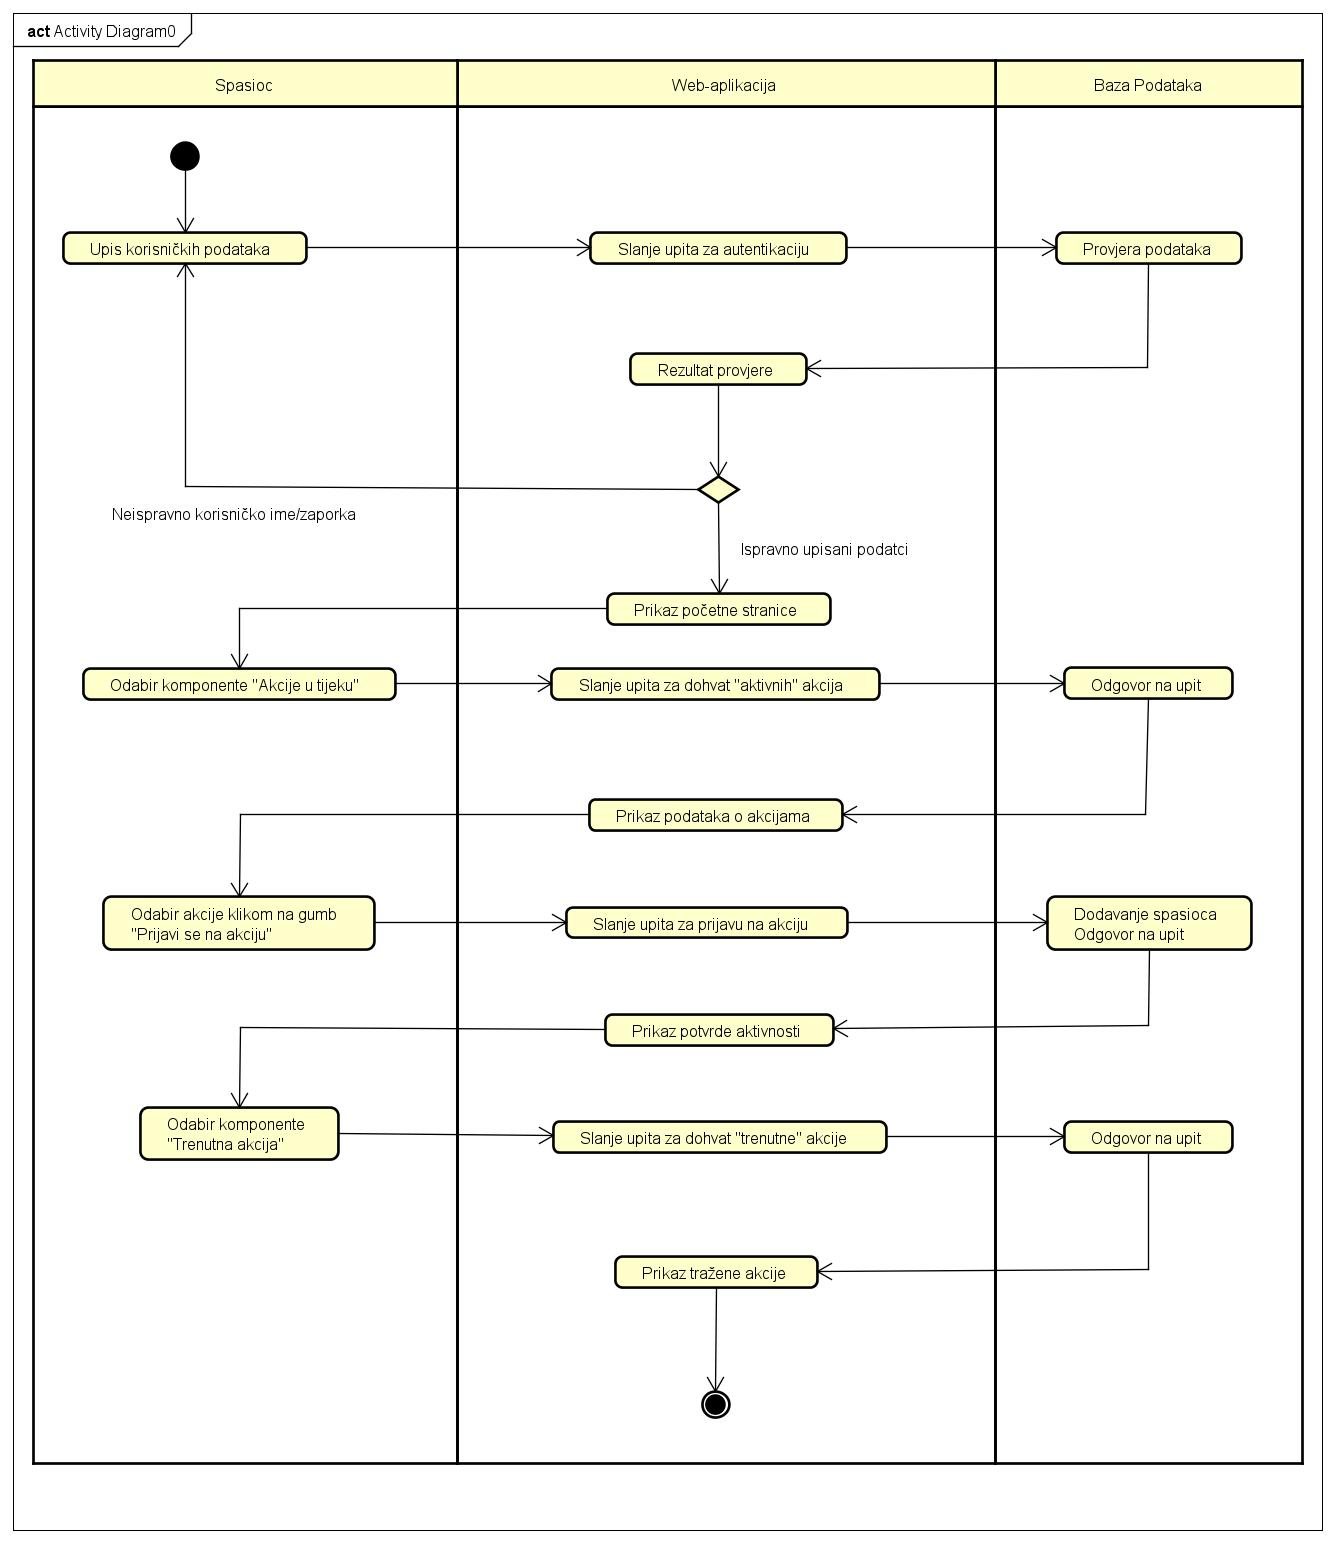
\includegraphics[width=\linewidth]{./slike/PrijavaNaAkciju.jpg}
			\caption{Prikaz dijagrama aktivnosti za javljanje spasioca na akciju}
			
		\end{figure}
		\eject
		
	\end{packed_item}
		\newpage
		\begin{packed_item}
			\begin{figure}[h!]
				
				\centering
				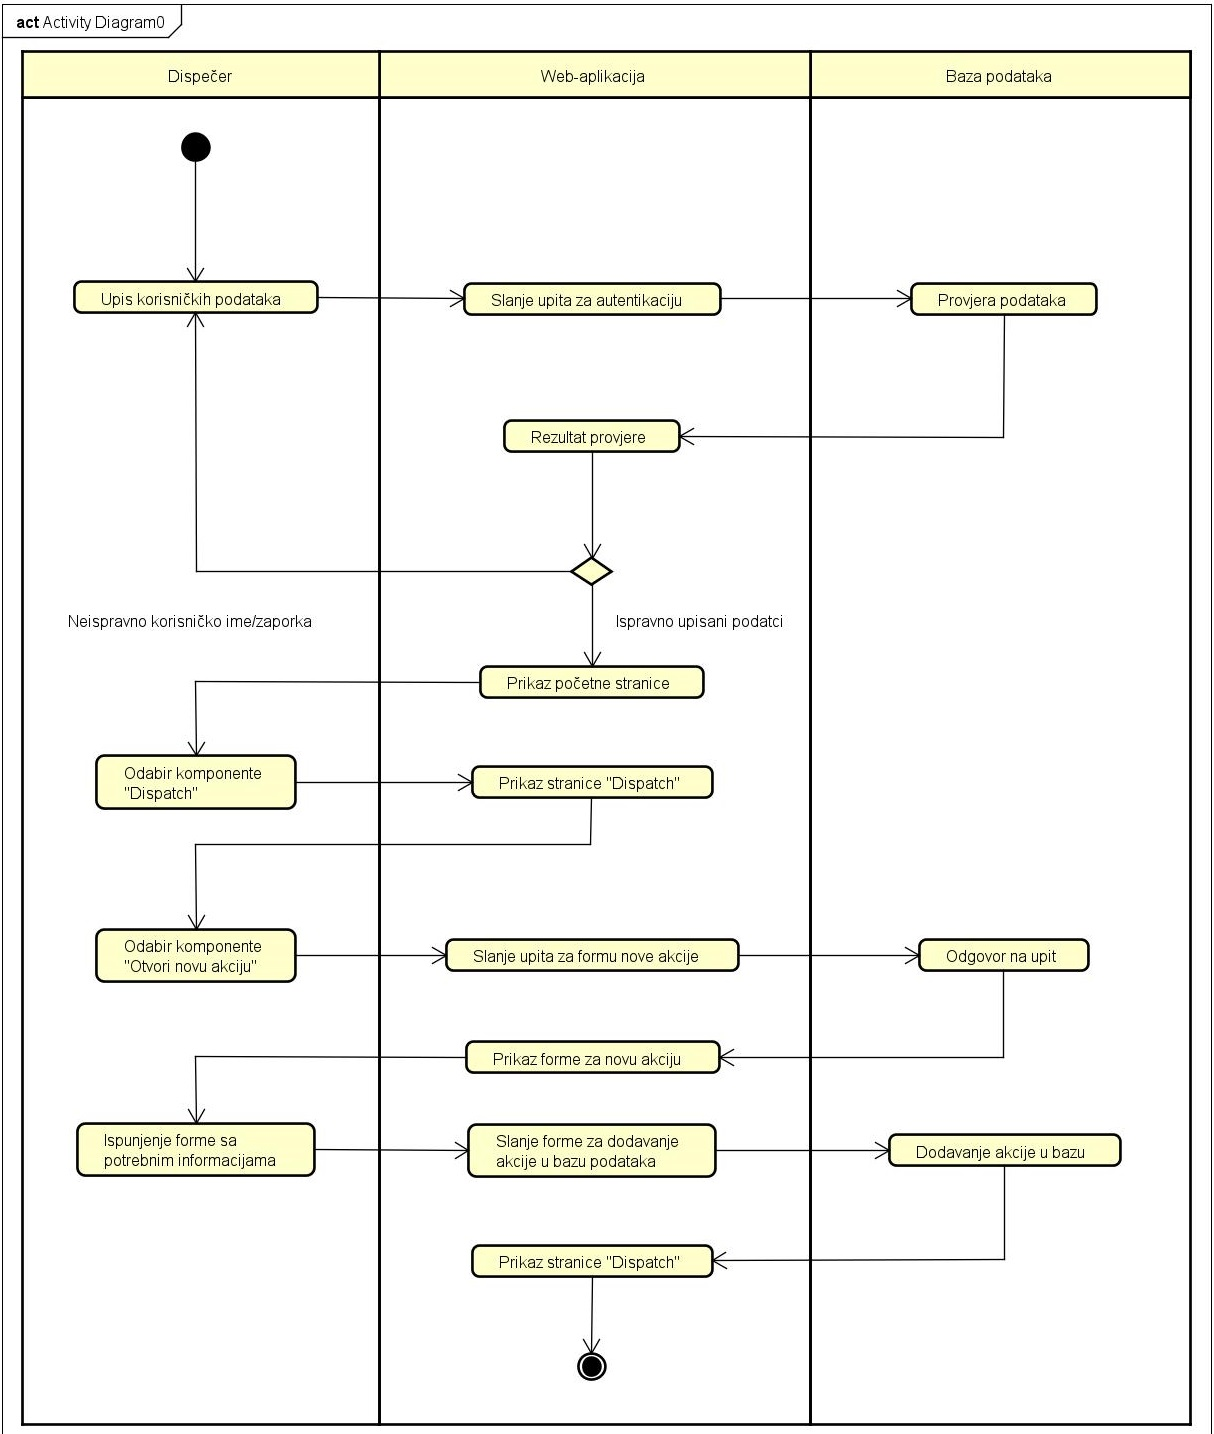
\includegraphics[width=\linewidth]{./slike/StvaranjeAkcije.jpg}
				\caption{Prikaz dijagrama aktivnosti za stvaranje nove akcije spašavanja}
			\end{figure}
			\eject
			
			\item {Slika 4.7 prikazuje proces stvaranja nove akcije spašavanja.Dispečer je dužan otvoriti karticu dispatch te klikom na gumb "Otvori novu akciju". Zatim mu se na upit šalje forma za ispunu informacija o novoj akciji i osobi. Pri završetku ispune forme akcija je dodana u bazu podataka te je dispečer vraćen na stranicu Dispatch.}\\
			
			
		\end{packed_item}
	\newpage

	\section{Dijagram komponenti}
	

		{Dijagram komponenti prikazan na slici dolje(slike 4.8) prikazuje organizaciju i međuovisnost komponenti, unutarnje strukture te odnose komponenata prema njihovoj okolini.Web-aplikaciji se pristupa pomoću dva sučelja. Koristimo sučelje za dohvat HTML,CSS i JS datoteka dobivamo datoteke vezane za \textit{frontend} dio aplikacije.Router je komponenta aplikacije koja na upis podataka ovisno o razini dozvola određuje koja datoteka će biti poslužena korisniku na sučelju. Svaki dio \textit{frontend} arhitekture raspoređen je u nekolicine JavaScript datoteka koje su raspodijeljene u logičke cjeline, neke od kojih su nazvane po kategoriji korisnika koji postoje u aplikaciji. Sve datoteke u našem projektu koje su oblika JavaScript ovise o \textbf{REACT} biblioteci preko koje dohvaćaju razne komponente potrebne za ispravan rad aplikacije,npr. gumbi,forme i sl.Preko sučelja \textbf{REST API} dohvaćaju se datoteke tipa JSON. \textbf{REST API} koristi za posluživanje \textit{backend} dijela podataka. Za poslugu podataka iz baze podataka koristi se \textbf{JPA} oblik podataka u datotekama te za upite u bazu.React-view komponenta pomoću svih navedenih sučelja komunicira za \textit{HGSSTracks} aplikacijom i s naputkom korisnikovih akcija na samoj aplikaciji osvježava prikaz ,prikazuje nove podatke koje je korisnik zatražio ili datoteke tj. upite koje je korisnik slao a vezane su za bazu podataka.}\\
		
		\begin{figure}[h!]
			\centering
			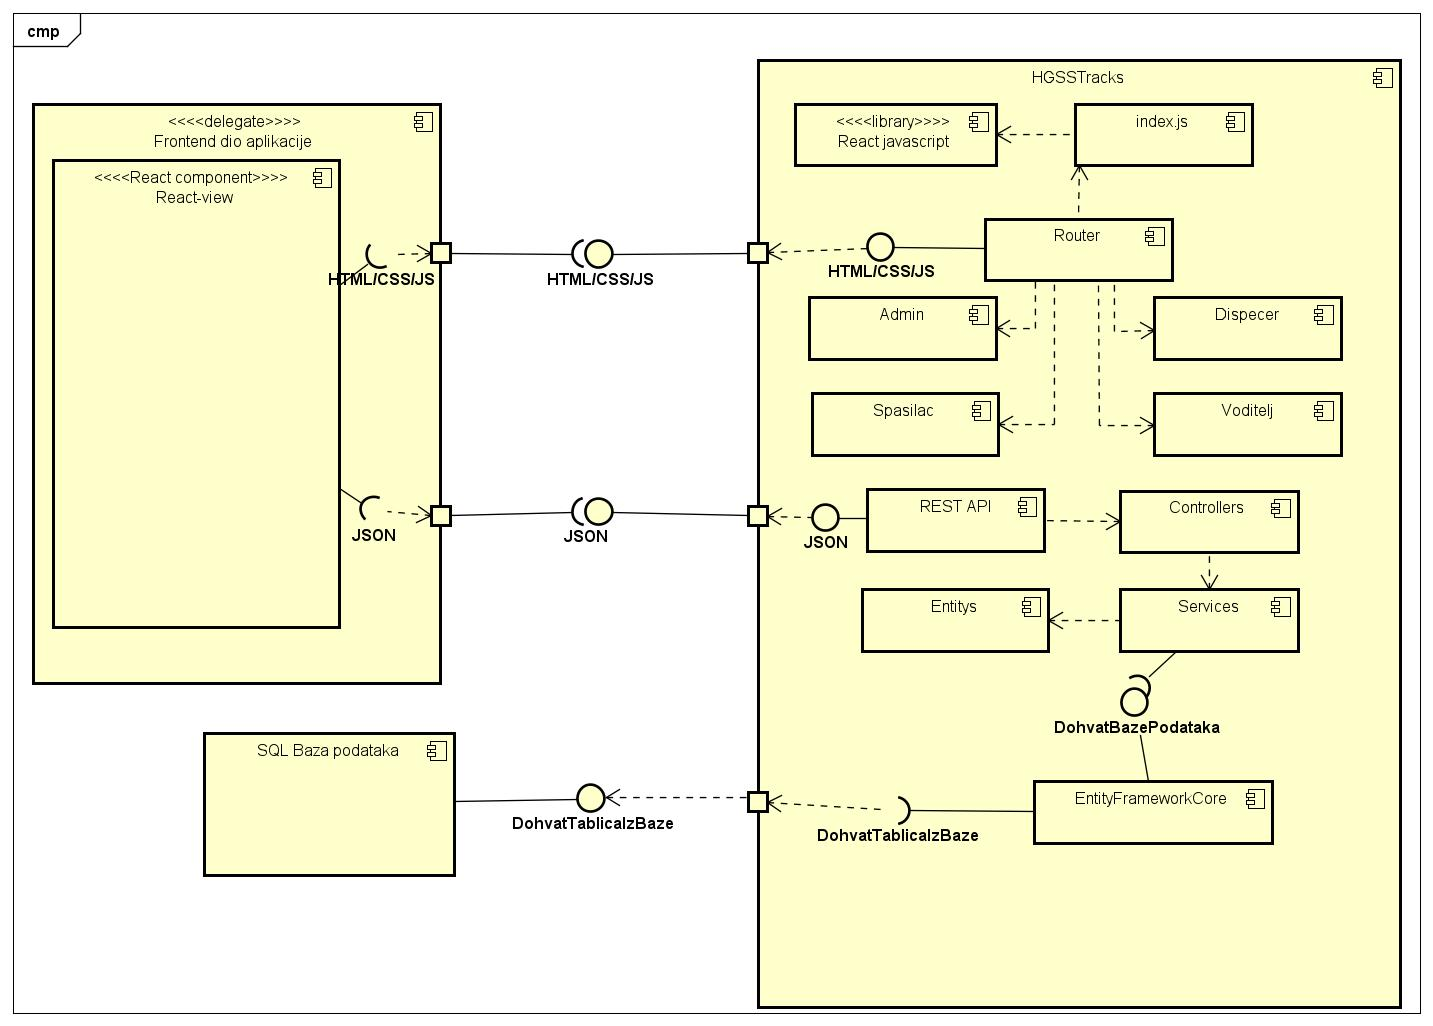
\includegraphics[width=\linewidth]{./slike/DijagramKomponenti.jpg}
			\caption{Prikaz dijagrama komponenti}
			
		\end{figure}